\documentclass[../tex_main/NEMO_manual]{subfiles}
\begin{document}
% ================================================================
% Chapter 2 ——— Space and Time Domain (DOM)
% ================================================================
\chapter{Space Domain (DOM)}
\label{chap:DOM}
\minitoc

% Missing things:
% 	- istate: description of the initial state   ==> this has to be put elsewhere..
%                  perhaps in MISC ?  By the way the initialisation of T S and dynamics 
%                  should be put outside of DOM routine (better with TRC staff and off-line
%                  tracers)
% 	-geo2ocean:  how to switch from geographic to mesh coordinate
%     - domclo:  closed sea and lakes.... management of closea sea area : specific to global configuration, both forced and coupled


\newpage
$\ $\newline    % force a new line

Having defined the continuous equations in \autoref{chap:PE} and chosen a time discretization \autoref{chap:STP},
we need to choose a discretization on a grid, and numerical algorithms.
In the present chapter, we provide a general description of the staggered grid used in \NEMO,
and other information relevant to the main directory routines as well as the DOM (DOMain) directory.

$\ $\newline    % force a new line

% ================================================================
% Fundamentals of the Discretisation
% ================================================================
\section{Fundamentals of the discretisation}
\label{sec:DOM_basics}

% -------------------------------------------------------------------------------------------------------------
%        Arrangement of Variables 
% -------------------------------------------------------------------------------------------------------------
\subsection{Arrangement of variables}
\label{subsec:DOM_cell}

%>>>>>>>>>>>>>>>>>>>>>>>>>>>>
\begin{figure}[!tb]    \begin{center}
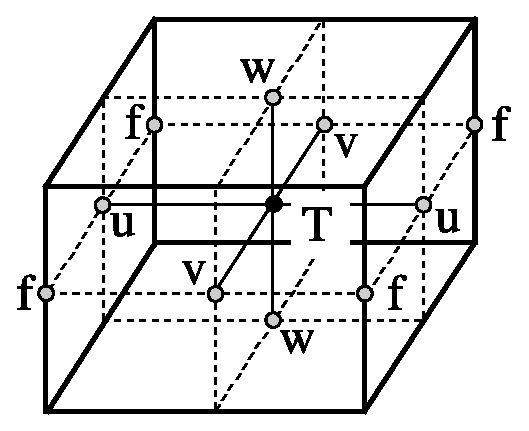
\includegraphics[width=0.90\textwidth]{Fig_cell}
\caption{ \protect\label{fig:cell}
  Arrangement of variables.
  $t$ indicates scalar points where temperature, salinity, density, pressure and horizontal divergence are defined.
  ($u$,$v$,$w$) indicates vector points,
  and $f$ indicates vorticity points where both relative and planetary vorticities are defined}
\end{center}   \end{figure}
%>>>>>>>>>>>>>>>>>>>>>>>>>>>>

The numerical techniques used to solve the Primitive Equations in this model are based on the traditional,
centred second-order finite difference approximation.
Special attention has been given to the homogeneity of the solution in the three space directions.
The arrangement of variables is the same in all directions.
It consists of cells centred on scalar points ($t$, $S$, $p$, $\rho$) with vector points $(u, v, w)$ defined in
the centre of each face of the cells (\autoref{fig:cell}).
This is the generalisation to three dimensions of the well-known ``C'' grid in Arakawa's classification
\citep{Mesinger_Arakawa_Bk76}.
The relative and planetary vorticity, $\zeta$ and $f$, are defined in the centre of each vertical edge and
the barotropic stream function $\psi$ is defined at horizontal points overlying the $\zeta$ and $f$-points.

The ocean mesh ($i.e.$ the position of all the scalar and vector points) is defined by
the transformation that gives ($\lambda$ ,$\varphi$ ,$z$) as a function of $(i,j,k)$.
The grid-points are located at integer or integer and a half value of $(i,j,k)$ as indicated on \autoref{tab:cell}.
In all the following, subscripts $u$, $v$, $w$, $f$, $uw$, $vw$ or $fw$ indicate the position of
the grid-point where the scale factors are defined.
Each scale factor is defined as the local analytical value provided by \autoref{eq:scale_factors}.
As a result,
the mesh on which partial derivatives $\frac{\partial}{\partial \lambda}, \frac{\partial}{\partial \varphi}$,
and $\frac{\partial}{\partial z} $ are evaluated is a uniform mesh with a grid size of unity.
Discrete partial derivatives are formulated by the traditional,
centred second order finite difference approximation while
the scale factors are chosen equal to their local analytical value.
An important point here is that the partial derivative of the scale factors must be evaluated by
centred finite difference approximation, not from their analytical expression.
This preserves the symmetry of the discrete set of equations and
therefore satisfies many of the continuous properties (see \autoref{apdx:C}).
A similar, related remark can be made about the domain size:
when needed, an area, volume, or the total ocean depth must be evaluated as the sum of the relevant scale factors
(see \autoref{eq:DOM_bar}) in the next section).

%>>>>>>>>>>>>>>>>>>>>>>>>>>>>
\begin{table}[!tb]
\begin{center} \begin{tabular}{|p{46pt}|p{56pt}|p{56pt}|p{56pt}|}
\hline
T	&$i$ 		& $j$		& $k$		 \\ \hline
u	& $i+1/2$	& $j$		& $k$	 	\\ \hline
v	& $i$	 	& $j+1/2$	& $k$	 	\\ \hline
w	& $i$	 	& $j$		& $k+1/2$ 	\\ \hline
f	& $i+1/2$ 	& $j+1/2$	& $k$	 	\\ \hline
uw	& $i+1/2$ 	& $j$		& $k+1/2$ 	\\ \hline
vw	& $i$	 	& $j+1/2$	& $k+1/2$ 	\\ \hline
fw	& $i+1/2$ 	& $j+1/2$	& $k+1/2$ 	\\ \hline
\end{tabular}
\caption{ \protect\label{tab:cell}
  Location of grid-points as a function of integer or integer and a half value of the column, line or level.
  This indexing is only used for the writing of the semi-discrete equation.
  In the code, the indexing uses integer values only and has a reverse direction in the vertical
  (see \autoref{subsec:DOM_Num_Index})}
\end{center}
\end{table}
%>>>>>>>>>>>>>>>>>>>>>>>>>>>>

% -------------------------------------------------------------------------------------------------------------
%        Vector Invariant Formulation 
% -------------------------------------------------------------------------------------------------------------
\subsection{Discrete operators}
\label{subsec:DOM_operators}

Given the values of a variable $q$ at adjacent points,
the differencing and averaging operators at the midpoint between them are:
\begin{subequations} \label{eq:di_mi}
\begin{align}
 \delta_i [q]       &=  \  \    q(i+1/2)  - q(i-1/2)		\\
 \overline q^{\,i} &= \left\{ q(i+1/2) + q(i-1/2) \right\} \; / \; 2
\end{align}
\end{subequations}

Similar operators are defined with respect to $i+1/2$, $j$, $j+1/2$, $k$, and $k+1/2$.
Following \autoref{eq:PE_grad} and \autoref{eq:PE_lap}, the gradient of a variable $q$ defined at
a $t$-point has its three components defined at $u$-, $v$- and $w$-points while
its Laplacien is defined at $t$-point.
These operators have the following discrete forms in the curvilinear $s$-coordinate system:
\begin{equation} \label{eq:DOM_grad}
\nabla q\equiv 	\frac{1}{e_{1u} } \delta_{i+1/2 } [q] \;\,\mathbf{i}
		+	\frac{1}{e_{2v} } \delta_{j+1/2 } [q] \;\,\mathbf{j}
		+	\frac{1}{e_{3w}} \delta_{k+1/2} [q] \;\,\mathbf{k}
\end{equation}
\begin{multline} \label{eq:DOM_lap}
\Delta q\equiv \frac{1}{e_{1t}\,e_{2t}\,e_{3t} }
       \;\left(          \delta_i  \left[ \frac{e_{2u}\,e_{3u}} {e_{1u}} \;\delta_{i+1/2} [q] \right]
+                        \delta_j  \left[ \frac{e_{1v}\,e_{3v}}  {e_{2v}} \;\delta_{j+1/2} [q] \right] \;  \right)		\\
+\frac{1}{e_{3t}} \delta_k \left[ \frac{1}{e_{3w} }                     \;\delta_{k+1/2} [q] \right]
\end{multline}

Following \autoref{eq:PE_curl} and \autoref{eq:PE_div}, a vector ${\rm {\bf A}}=\left( a_1,a_2,a_3\right)$
defined at vector points $(u,v,w)$ has its three curl components defined at $vw$-, $uw$, and $f$-points,
and its divergence defined at $t$-points:
\begin{align}  \label{eq:DOM_curl}
 \nabla \times {\rm{\bf A}}\equiv &
      \frac{1}{e_{2v}\,e_{3vw} } \ \left( \delta_{j +1/2} \left[e_{3w}\,a_3 \right] -\delta_{k+1/2} \left[e_{2v} \,a_2 \right] \right)  &\ \mathbf{i} \\ 
 +& \frac{1}{e_{2u}\,e_{3uw}} \ \left( \delta_{k+1/2} \left[e_{1u}\,a_1  \right] -\delta_{i +1/2} \left[e_{3w}\,a_3 \right] \right)  &\ \mathbf{j} \\
 +& \frac{1}{e_{1f} \,e_{2f}    } \ \left( \delta_{i +1/2} \left[e_{2v}\,a_2  \right] -\delta_{j +1/2} \left[e_{1u}\,a_1 \right] \right)  &\ \mathbf{k}
 \end{align}
\begin{align} \label{eq:DOM_div}
\nabla \cdot \rm{\bf A} \equiv 
    \frac{1}{e_{1t}\,e_{2t}\,e_{3t}} \left( \delta_i \left[e_{2u}\,e_{3u}\,a_1 \right]
                                           +\delta_j \left[e_{1v}\,e_{3v}\,a_2 \right] \right)+\frac{1}{e_{3t} }\delta_k \left[a_3 \right]
\end{align}

The vertical average over the whole water column denoted by an overbar becomes for a quantity $q$ which
is a masked field (i.e. equal to zero inside solid area):
\begin{equation} \label{eq:DOM_bar}
\bar q 	=         \frac{1}{H}    \int_{k^b}^{k^o} {q\;e_{3q} \,dk} 
		\equiv \frac{1}{H_q }\sum\limits_k {q\;e_{3q} }
\end{equation}
where $H_q$  is the ocean depth, which is the masked sum of the vertical scale factors at $q$ points,
$k^b$ and $k^o$ are the bottom and surface $k$-indices,
and the symbol $k^o$ refers to a summation over all grid points of the same type in the direction indicated by
the subscript (here $k$). 

In continuous form, the following properties are satisfied:
\begin{equation} \label{eq:DOM_curl_grad}
\nabla \times \nabla q ={\rm {\bf {0}}}
\end{equation}
\begin{equation} \label{eq:DOM_div_curl}
\nabla \cdot \left( {\nabla \times {\rm {\bf A}}} \right)=0
\end{equation}

It is straightforward to demonstrate that these properties are verified locally in discrete form as soon as
the scalar $q$ is taken at $t$-points and
the vector \textbf{A} has its components defined at vector points $(u,v,w)$.

Let $a$ and $b$ be two fields defined on the mesh, with value zero inside continental area.
Using integration by parts it can be shown that
the differencing operators ($\delta_i$, $\delta_j$ and $\delta_k$) are skew-symmetric linear operators,
and further that the averaging operators $\overline{\,\cdot\,}^{\,i}$, $\overline{\,\cdot\,}^{\,k}$ and
$\overline{\,\cdot\,}^{\,k}$) are symmetric linear operators,
$i.e.$
\begin{align} 
\label{eq:DOM_di_adj}
\sum\limits_i { a_i \;\delta_i \left[ b \right]} 
	&\equiv -\sum\limits_i {\delta_{i+1/2} \left[ a \right]\;b_{i+1/2} }      \\
\label{eq:DOM_mi_adj}
\sum\limits_i { a_i \;\overline b^{\,i}} 
	& \equiv \quad \sum\limits_i {\overline a ^{\,i+1/2}\;b_{i+1/2} } 
\end{align}

In other words, the adjoint of the differencing and averaging operators are $\delta_i^*=\delta_{i+1/2}$ and 
${(\overline{\,\cdot \,}^{\,i})}^*= \overline{\,\cdot\,}^{\,i+1/2}$, respectively. 
These two properties will be used extensively in the \autoref{apdx:C} to
demonstrate integral conservative properties of the discrete formulation chosen.

% -------------------------------------------------------------------------------------------------------------
%        Numerical Indexing 
% -------------------------------------------------------------------------------------------------------------
\subsection{Numerical indexing}
\label{subsec:DOM_Num_Index}

%>>>>>>>>>>>>>>>>>>>>>>>>>>>>
\begin{figure}[!tb]  \begin{center}
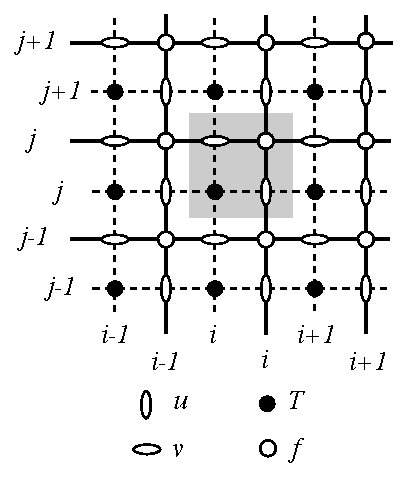
\includegraphics[width=0.90\textwidth]{Fig_index_hor}
\caption{   \protect\label{fig:index_hor}
  Horizontal integer indexing used in the \textsc{Fortran} code.
  The dashed area indicates the cell in which variables contained in arrays have the same $i$- and $j$-indices}
\end{center}   \end{figure}
%>>>>>>>>>>>>>>>>>>>>>>>>>>>>

The array representation used in the \textsc{Fortran} code requires an integer indexing while
the analytical definition of the mesh (see \autoref{subsec:DOM_cell}) is associated with the use of
integer values for $t$-points and both integer and integer and a half values for all the other points.
Therefore a specific integer indexing must be defined for points other than $t$-points
($i.e.$ velocity and vorticity grid-points).
Furthermore, the direction of the vertical indexing has been changed so that the surface level is at $k=1$.

% -----------------------------------
%        Horizontal Indexing 
% -----------------------------------
\subsubsection{Horizontal indexing}
\label{subsec:DOM_Num_Index_hor}

The indexing in the horizontal plane has been chosen as shown in \autoref{fig:index_hor}.
For an increasing $i$ index ($j$ index),
the $t$-point and the eastward $u$-point (northward $v$-point) have the same index
(see the dashed area in \autoref{fig:index_hor}).
A $t$-point and its nearest northeast $f$-point have the same $i$-and $j$-indices.

% -----------------------------------
%        Vertical indexing 
% -----------------------------------
\subsubsection{Vertical indexing}
\label{subsec:DOM_Num_Index_vertical}

In the vertical, the chosen indexing requires special attention since
the $k$-axis is re-orientated downward in the \textsc{Fortran} code compared to
the indexing used in the semi-discrete equations and given in \autoref{subsec:DOM_cell}.
The sea surface corresponds to the $w$-level $k=1$ which is the same index as $t$-level just below
(\autoref{fig:index_vert}).
The last $w$-level ($k=jpk$) either corresponds to the ocean floor or is inside the bathymetry while
the last $t$-level is always inside the bathymetry (\autoref{fig:index_vert}).
Note that for an increasing $k$ index, a $w$-point and the $t$-point just below have the same $k$ index,
in opposition to what is done in the horizontal plane where
it is the $t$-point and the nearest velocity points in the direction of the horizontal axis that
have the same $i$ or $j$ index
(compare the dashed area in \autoref{fig:index_hor} and \autoref{fig:index_vert}).
Since the scale factors are chosen to be strictly positive, a \emph{minus sign} appears in the \textsc{Fortran} 
code \emph{before all the vertical derivatives} of the discrete equations given in this documentation.

%>>>>>>>>>>>>>>>>>>>>>>>>>>>>
\begin{figure}[!pt]    \begin{center}
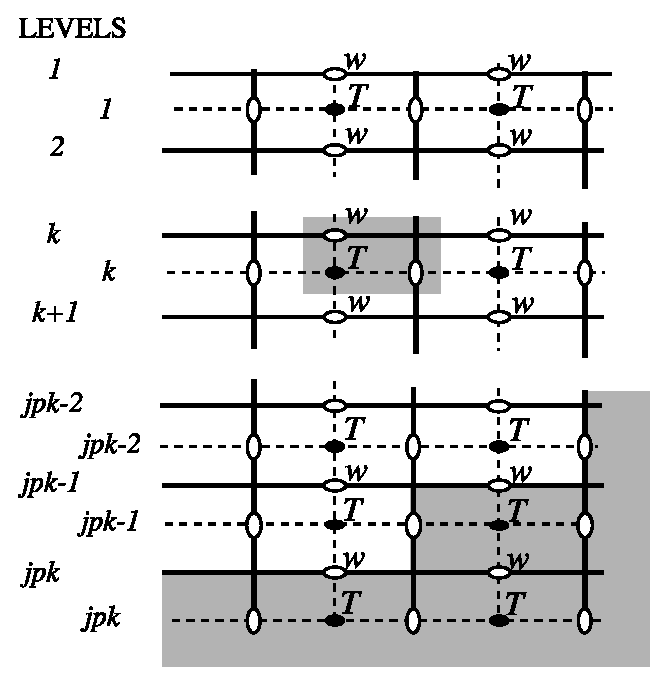
\includegraphics[width=.90\textwidth]{Fig_index_vert}
\caption{ \protect\label{fig:index_vert}
  Vertical integer indexing used in the \textsc{Fortran } code.
  Note that the $k$-axis is orientated downward.
  The dashed area indicates the cell in which variables contained in arrays have the same $k$-index.}
\end{center}   \end{figure}
%>>>>>>>>>>>>>>>>>>>>>>>>>>>>

% -----------------------------------
%        Domain Size
% -----------------------------------
\subsubsection{Domain size}
\label{subsec:DOM_size}

The total size of the computational domain is set by the parameters \np{jpiglo},
\np{jpjglo} and \np{jpkglo} in the $i$, $j$ and $k$ directions respectively.
%%%
%%%
%%%
Parameters $jpi$ and $jpj$ refer to the size of each processor subdomain when
the code is run in parallel using domain decomposition (\key{mpp\_mpi} defined,
see \autoref{sec:LBC_mpp}).


$\ $\newline    % force a new line

% ================================================================
% Domain: List of fields needed
% ================================================================
\section{Needed fields}
\label{sec:DOM_fields}
The ocean mesh ($i.e.$ the position of all the scalar and vector points) is defined by the transformation that gives $(\lambda,\varphi,z)$ as a function of $(i,j,k)$.
The grid-points are located at integer or integer and a half values of as indicated in \autoref{tab:cell}.
The associated scale factors are defined using the analytical first derivative of the transformation
\autoref{eq:scale_factors}.
Necessary fields for configuration definition are: \\
Geographic position :

longitude: glamt, glamu, glamv and glamf (at T, U, V and F point)

latitude: gphit, gphiu, gphiv and gphif (at T, U, V and F point)\\
Coriolis parameter (if domain not on the sphere): 

 ff\_f  and  ff\_t (at T and F point)\\
Scale factors : 
 
 e1t, e1u, e1v and e1f (on i direction),

 e2t, e2u, e2v and e2f (on j direction) and

 ie1e2u\_v, e1e2u , e1e2v   
 
e1e2u , e1e2v are u and v surfaces (if gridsize reduction in some straits)\\
ie1e2u\_v is a flag to flag set u and  v surfaces are neither read nor computed.\\
 
These fields can be read in an domain input file which name is setted in
\np{cn\_domcfg} parameter specified in \ngn{namcfg}.

\nlst{namcfg}
or they can be defined in an analytical way in MY\_SRC directory of the configuration.
For Reference Configurations of NEMO input domain files are supplied by NEMO System Team.
For analytical definition of input fields two routines are supplied: \mdl{userdef\_hgr} and \mdl{userdef\_zgr}.
They are an example of GYRE configuration parameters, and they are available in NEMO/OPA\_SRC/USR directory,
they provide the horizontal and vertical mesh. 
% -------------------------------------------------------------------------------------------------------------
%        Needed fields 
% -------------------------------------------------------------------------------------------------------------
%\subsection{List of needed fields to build DOMAIN}
%\label{subsec:DOM_fields_list}


% ================================================================
% Domain: Horizontal Grid (mesh) 
% ================================================================
\section{Horizontal grid mesh (\protect\mdl{domhgr})}
\label{sec:DOM_hgr}

% -------------------------------------------------------------------------------------------------------------
%        Coordinates and scale factors 
% -------------------------------------------------------------------------------------------------------------
\subsection{Coordinates and scale factors}
\label{subsec:DOM_hgr_coord_e}

The ocean mesh ($i.e.$ the position of all the scalar and vector points) is defined by
the transformation that gives $(\lambda,\varphi,z)$ as a function of $(i,j,k)$.
The grid-points are located at integer or integer and a half values of as indicated in \autoref{tab:cell}.
The associated scale factors are defined using the analytical first derivative of the transformation
\autoref{eq:scale_factors}.
These definitions are done in two modules, \mdl{domhgr} and \mdl{domzgr},
which provide the horizontal and vertical meshes, respectively.
This section deals with the horizontal mesh parameters.

In a horizontal plane, the location of all the model grid points is defined from
the analytical expressions of the longitude $\lambda$ and latitude $\varphi$ as a function of $(i,j)$.
The horizontal scale factors are calculated using \autoref{eq:scale_factors}.
For example, when the longitude and latitude are function of a single value
($i$ and $j$, respectively) (geographical configuration of the mesh),
the horizontal mesh definition reduces to define the wanted $\lambda(i)$, $\varphi(j)$,
and their derivatives $\lambda'(i)$ $\varphi'(j)$ in the \mdl{domhgr} module.
The model computes the grid-point positions and scale factors in the horizontal plane as follows:
\begin{flalign*}
\lambda_t &\equiv \text{glamt}= \lambda(i)	  & \varphi_t &\equiv \text{gphit} = \varphi(j)\\
\lambda_u &\equiv \text{glamu}= \lambda(i+1/2)& \varphi_u &\equiv \text{gphiu}= \varphi(j)\\
\lambda_v &\equiv \text{glamv}= \lambda(i)       & \varphi_v &\equiv \text{gphiv} = \varphi(j+1/2)\\
\lambda_f &\equiv \text{glamf }= \lambda(i+1/2)& \varphi_f &\equiv \text{gphif }= \varphi(j+1/2) 
\end{flalign*}
\begin{flalign*}
e_{1t} &\equiv \text{e1t} = r_a |\lambda'(i)		\; \cos\varphi(j)  |&
e_{2t} &\equiv \text{e2t} = r_a |\varphi'(j)|  \\
e_{1u} &\equiv \text{e1t} = r_a |\lambda'(i+1/2)	\; \cos\varphi(j)  |&
e_{2u} &\equiv \text{e2t} = r_a |\varphi'(j)|\\
e_{1v} &\equiv \text{e1t} = r_a |\lambda'(i)		\; \cos\varphi(j+1/2)  |&
e_{2v} &\equiv \text{e2t} = r_a |\varphi'(j+1/2)|\\
e_{1f} &\equiv \text{e1t} = r_a |\lambda'(i+1/2)\; \cos\varphi(j+1/2)  |&
e_{2f} &\equiv \text{e2t} = r_a |\varphi'(j+1/2)|
\end{flalign*}
where the last letter of each computational name indicates the grid point considered and
$r_a$ is the earth radius (defined in \mdl{phycst} along with all universal constants).
Note that the horizontal position of and scale factors at $w$-points are exactly equal to those of $t$-points,
thus no specific arrays are defined at $w$-points. 

Note that the definition of the scale factors
($i.e.$ as the analytical first derivative of the transformation that
gives $(\lambda,\varphi,z)$ as a function of $(i,j,k)$)
is specific to the \NEMO model \citep{Marti_al_JGR92}.
As an example, $e_{1t}$ is defined locally at a $t$-point,
whereas many other models on a C grid choose to define such a scale factor as
the distance between the $U$-points on each side of the $t$-point.
Relying on an analytical transformation has two advantages:
firstly, there is no ambiguity in the scale factors appearing in the discrete equations,
since they are first introduced in the continuous equations;
secondly, analytical transformations encourage good practice by the definition of smoothly varying grids
(rather than allowing the user to set arbitrary jumps in thickness between adjacent layers) \citep{Treguier1996}.
An example of the effect of such a choice is shown in \autoref{fig:zgr_e3}.
%>>>>>>>>>>>>>>>>>>>>>>>>>>>>
\begin{figure}[!t]     \begin{center}
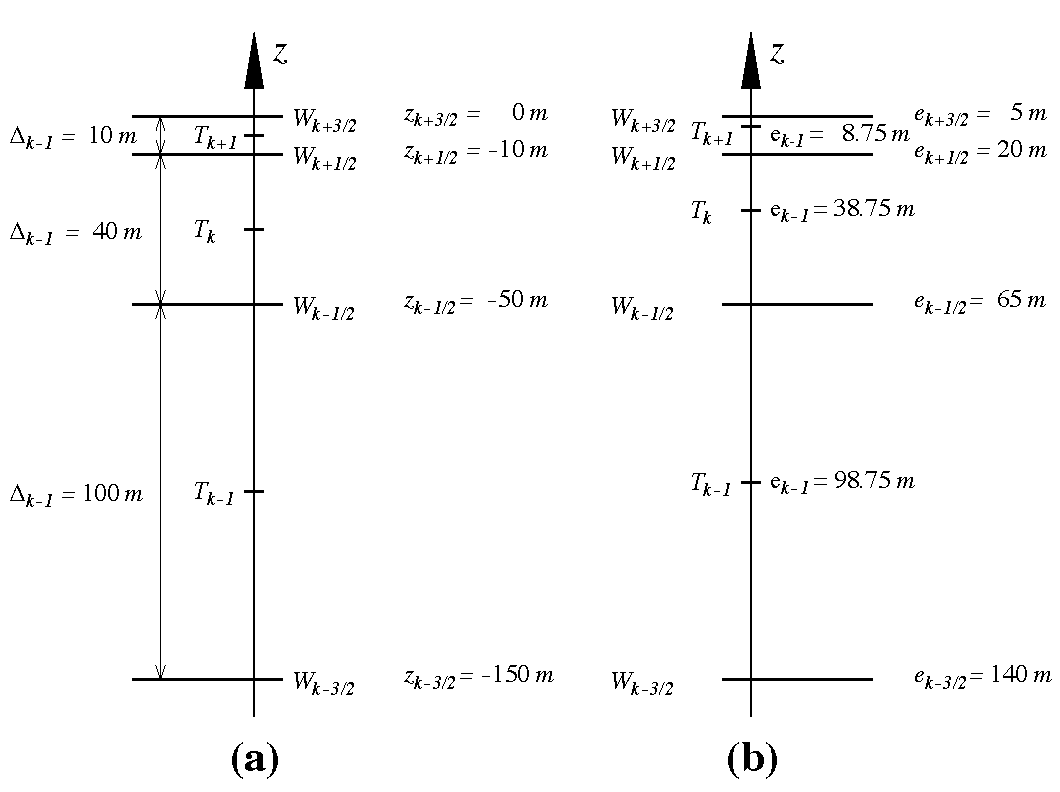
\includegraphics[width=0.90\textwidth]{Fig_zgr_e3}
\caption{ \protect\label{fig:zgr_e3}
  Comparison of (a) traditional definitions of grid-point position and grid-size in the vertical,
  and (b) analytically derived grid-point position and scale factors.
  For both grids here,
  the same $w$-point depth has been chosen but in (a) the $t$-points are set half way between $w$-points while
  in (b) they are defined from an analytical function: $z(k)=5\,(k-1/2)^3 - 45\,(k-1/2)^2 + 140\,(k-1/2) - 150$.
  Note the resulting difference between the value of the grid-size $\Delta_k$ and those of the scale factor $e_k$. }
\end{center}   \end{figure}
%>>>>>>>>>>>>>>>>>>>>>>>>>>>>

% -------------------------------------------------------------------------------------------------------------
%        Choice of horizontal grid
% -------------------------------------------------------------------------------------------------------------
\subsection{Choice of horizontal grid}
\label{subsec:DOM_hgr_msh_choice}


% -------------------------------------------------------------------------------------------------------------
%        Grid files
% -------------------------------------------------------------------------------------------------------------
\subsection{Output grid files}
\label{subsec:DOM_hgr_files}

All the arrays relating to a particular ocean model configuration (grid-point position, scale factors, masks)
can be saved in files if \np{nn\_msh} $\not= 0$ (namelist variable in \ngn{namdom}).
This can be particularly useful for plots and off-line diagnostics.
In some cases, the user may choose to make a local modification of a scale factor in the code.
This is the case in global configurations when restricting the width of a specific strait
(usually a one-grid-point strait that happens to be too wide due to insufficient model resolution).
An example is Gibraltar Strait in the ORCA2 configuration.
When such modifications are done,
the output grid written when \np{nn\_msh} $\not= 0$ is no more equal to the input grid.

$\ $\newline    % force a new line

% ================================================================
% Domain: Vertical Grid (domzgr)
% ================================================================
\section{Vertical grid (\protect\mdl{domzgr})}
\label{sec:DOM_zgr}
%-----------------------------------------nam_zgr & namdom-------------------------------------------
%
%\nlst{namzgr} 

\nlst{namdom} 
%-------------------------------------------------------------------------------------------------------------

Variables are defined through the \ngn{namzgr} and \ngn{namdom} namelists.
In the vertical, the model mesh is determined by four things: 
(1) the bathymetry given in meters; 
(2) the number of levels of the model (\jp{jpk}); 
(3) the analytical transformation $z(i,j,k)$ and the vertical scale factors (derivatives of the transformation); and
(4) the masking system, $i.e.$ the number of wet model levels at each 
$(i,j)$ column of points.

%>>>>>>>>>>>>>>>>>>>>>>>>>>>>
\begin{figure}[!tb]    \begin{center}
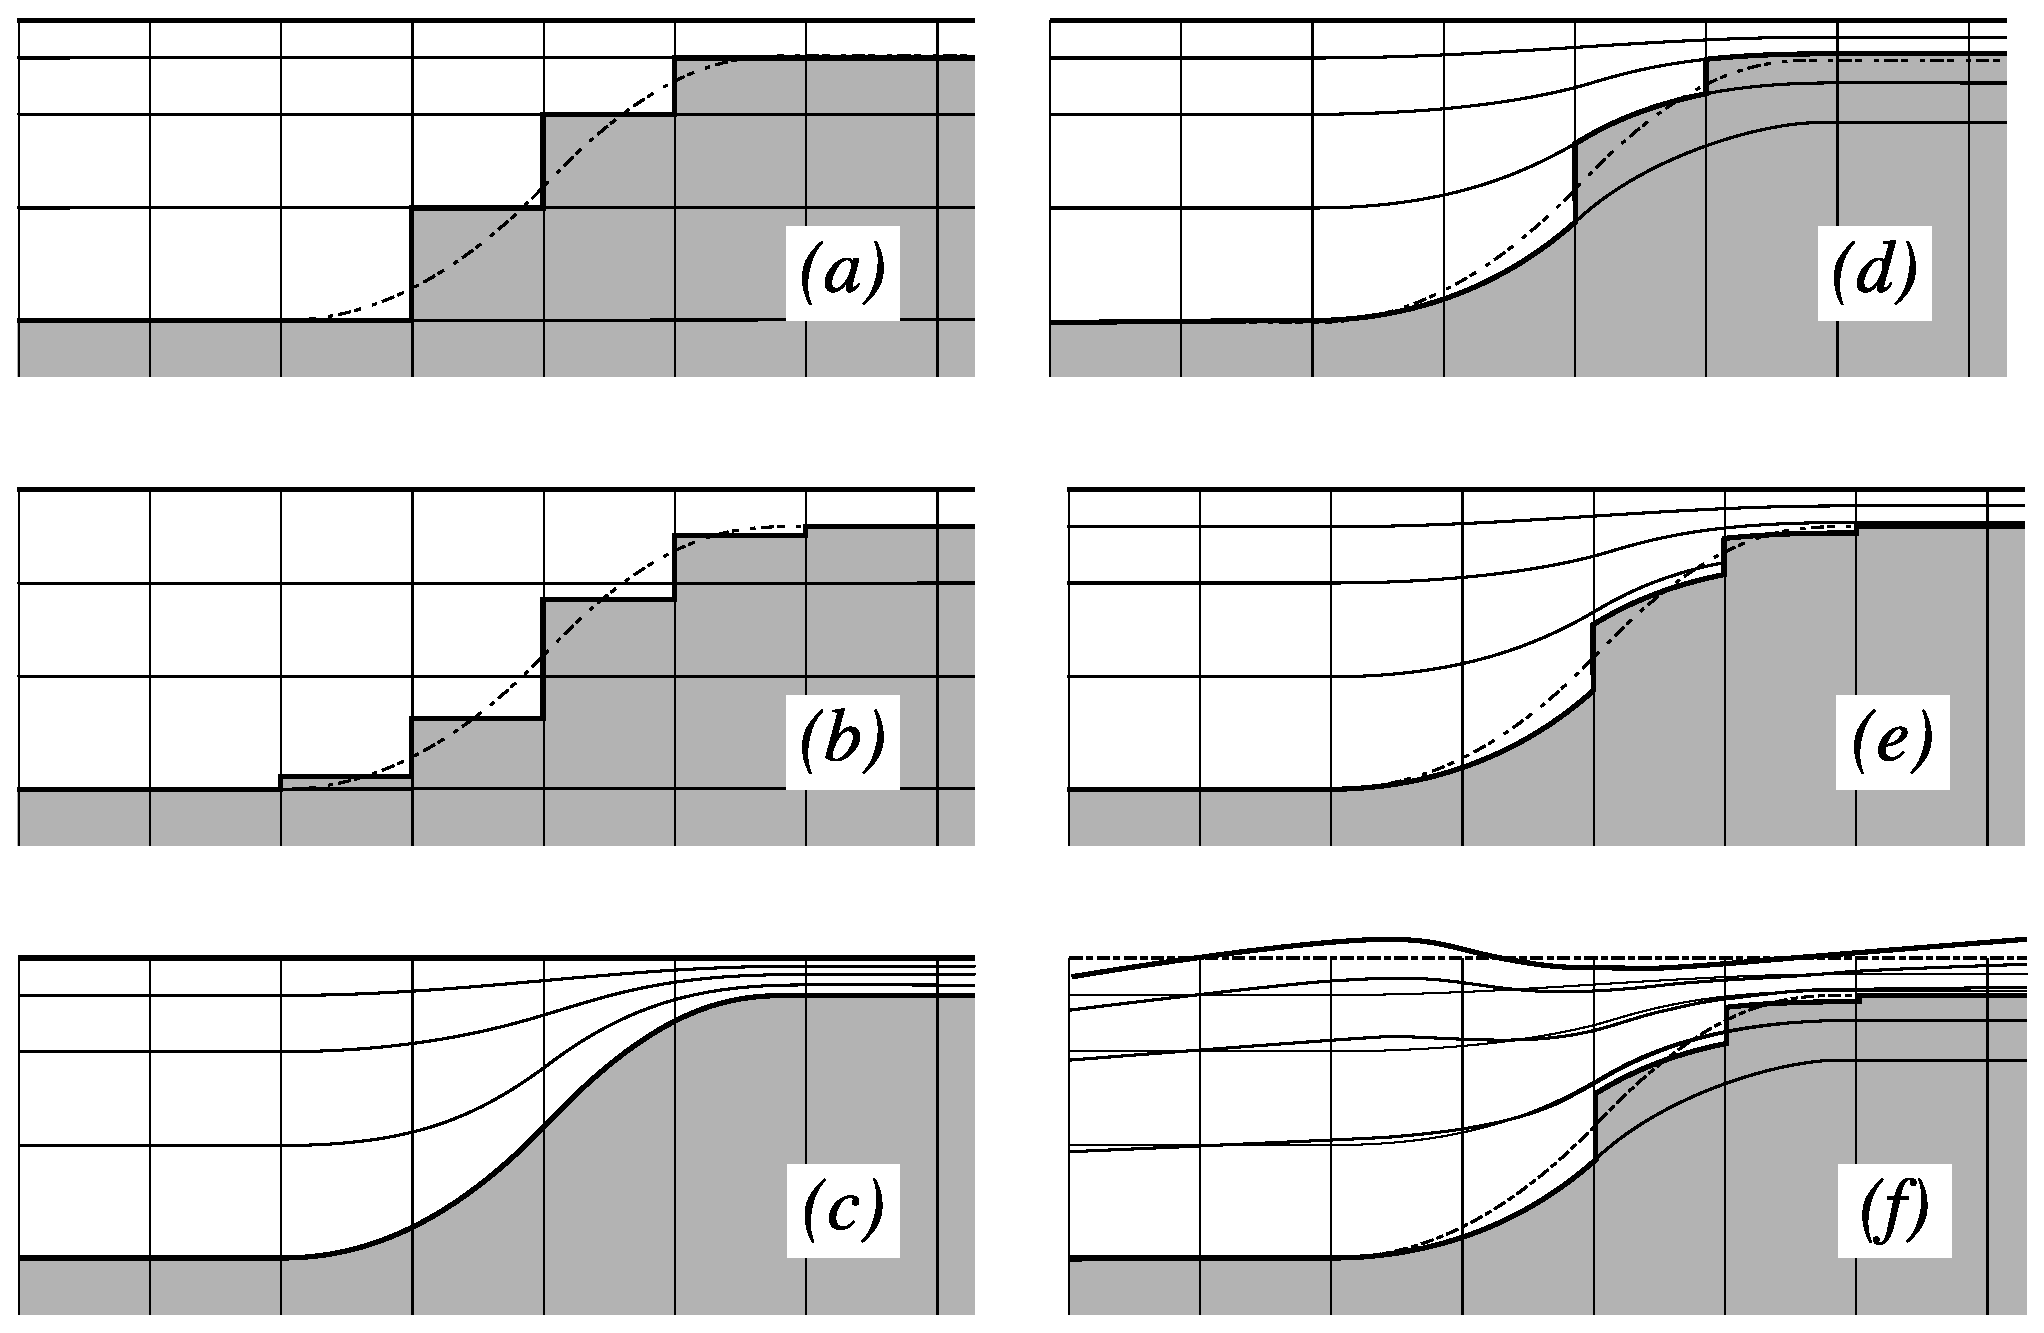
\includegraphics[width=1.0\textwidth]{Fig_z_zps_s_sps}
\caption{  \protect\label{fig:z_zps_s_sps}
  The ocean bottom as seen by the model:
  (a) $z$-coordinate with full step,
  (b) $z$-coordinate with partial step,
  (c) $s$-coordinate: terrain following representation,
  (d) hybrid $s-z$ coordinate,
  (e) hybrid $s-z$ coordinate with partial step, and
  (f) same as (e) but in the non-linear free surface (\protect\np{ln\_linssh}\forcode{ = .false.}).
  Note that the non-linear free surface can be used with any of the 5 coordinates (a) to (e).}
\end{center}   \end{figure}
%>>>>>>>>>>>>>>>>>>>>>>>>>>>>

The choice of a vertical coordinate, even if it is made through \ngn{namzgr} namelist parameters, 
must be done once of all at the beginning of an experiment.
It is not intended as an option which can be enabled or disabled in the middle of an experiment.
Three main choices are offered (\autoref{fig:z_zps_s_sps}a to c):
$z$-coordinate with full step bathymetry (\np{ln\_zco}\forcode{ = .true.}),
$z$-coordinate with partial step bathymetry (\np{ln\_zps}\forcode{ = .true.}),
or generalized, $s$-coordinate (\np{ln\_sco}\forcode{ = .true.}).
Hybridation of the three main coordinates are available:
$s-z$ or $s-zps$ coordinate (\autoref{fig:z_zps_s_sps} and \autoref{fig:z_zps_s_sps}e).
By default a non-linear free surface is used: the coordinate follow the time-variation of the free surface so that
the transformation is time dependent: $z(i,j,k,t)$ (\autoref{fig:z_zps_s_sps}f).
When a linear free surface is assumed (\np{ln\_linssh}\forcode{ = .true.}),
the vertical coordinate are fixed in time, but the seawater can move up and down across the z=0 surface
(in other words, the top of the ocean in not a rigid-lid). 
The last choice in terms of vertical coordinate concerns the presence (or not) in
the model domain of ocean cavities beneath ice shelves.
Setting \np{ln\_isfcav} to true allows to manage ocean cavities, otherwise they are filled in.
This option is currently only available in $z$- or $zps$-coordinate,
and partial step are also applied at the ocean/ice shelf interface.

Contrary to the horizontal grid, the vertical grid is computed in the code and
no provision is made for reading it from a file.
The only input file is the bathymetry (in meters) (\ifile{bathy\_meter})
\footnote{
  N.B. in full step $z$-coordinate, a \ifile{bathy\_level} file can replace the \ifile{bathy\_meter} file,
  so that the computation of the number of wet ocean point in each water column is by-passed}. 
If \np{ln\_isfcav}\forcode{ = .true.},
an extra file input file describing the ice shelf draft (in meters) (\ifile{isf\_draft\_meter}) is needed.

After reading the bathymetry, the algorithm for vertical grid definition differs between the different options:
\begin{description}
\item[\textit{zco}]
  set a reference coordinate transformation $z_0 (k)$, and set $z(i,j,k,t)=z_0 (k)$.
\item[\textit{zps}]
  set a reference coordinate transformation $z_0 (k)$,
  and calculate the thickness of the deepest level at each $(i,j)$ point using the bathymetry,
  to obtain the final three-dimensional depth and scale factor arrays.
\item[\textit{sco}]
  smooth the bathymetry to fulfil the hydrostatic consistency criteria and
  set the three-dimensional transformation.
\item[\textit{s-z} and \textit{s-zps}]
  smooth the bathymetry to fulfil the hydrostatic consistency criteria and
  set the three-dimensional transformation $z(i,j,k)$,
  and possibly introduce masking of extra land points to better fit the original bathymetry file.
\end{description}
%%%
\gmcomment{   add the description of the smoothing:  envelop topography...}
%%%

Unless a linear free surface is used (\np{ln\_linssh}\forcode{ = .false.}),
the arrays describing the grid point depths and vertical scale factors are three set of
three dimensional arrays $(i,j,k)$ defined at \textit{before}, \textit{now} and \textit{after} time step.
The time at which they are defined is indicated by a suffix:$\_b$, $\_n$, or $\_a$, respectively.
They are updated at each model time step using a fixed reference coordinate system which
computer names have a $\_0$ suffix.
When the linear free surface option is used (\np{ln\_linssh}\forcode{ = .true.}),
\textit{before}, \textit{now} and \textit{after} arrays are simply set one for all to their reference counterpart. 


% -------------------------------------------------------------------------------------------------------------
%        Meter Bathymetry
% -------------------------------------------------------------------------------------------------------------
\subsection{Meter bathymetry}
\label{subsec:DOM_bathy}

Three options are possible for defining the bathymetry, according to the namelist variable \np{nn\_bathy}
(found in \ngn{namdom} namelist): 
\begin{description}
\item[\np{nn\_bathy}\forcode{ = 0}]:
  a flat-bottom domain is defined.
  The total depth $z_w (jpk)$ is given by the coordinate transformation.
  The domain can either be a closed basin or a periodic channel depending on the parameter \np{jperio}. 
\item[\np{nn\_bathy}\forcode{ = -1}]:
  a domain with a bump of topography one third of the domain width at the central latitude.
  This is meant for the "EEL-R5" configuration, a periodic or open boundary channel with a seamount. 
\item[\np{nn\_bathy}\forcode{ = 1}]:
  read a bathymetry and ice shelf draft (if needed).
  The \ifile{bathy\_meter} file (Netcdf format) provides the ocean depth (positive, in meters) at
  each grid point of the model grid.
  The bathymetry is usually built by interpolating a standard bathymetry product ($e.g.$ ETOPO2) onto
  the horizontal ocean mesh.
  Defining the bathymetry also defines the coastline: where the bathymetry is zero,
  no model levels are defined (all levels are masked).

  The \ifile{isfdraft\_meter} file (Netcdf format) provides the ice shelf draft (positive, in meters) at
  each grid point of the model grid.
  This file is only needed if \np{ln\_isfcav}\forcode{ = .true.}.
  Defining the ice shelf draft will also define the ice shelf edge and the grounding line position.
\end{description}

When a global ocean is coupled to an atmospheric model it is better to represent all large water bodies
(e.g, great lakes, Caspian sea...)
even if the model resolution does not allow their communication with the rest of the ocean.
This is unnecessary when the ocean is forced by fixed atmospheric conditions,
so these seas can be removed from the ocean domain.
The user has the option to set the bathymetry in closed seas to zero (see \autoref{sec:MISC_closea}),
but the code has to be adapted to the user's configuration. 

% -------------------------------------------------------------------------------------------------------------
%        z-coordinate  and reference coordinate transformation
% -------------------------------------------------------------------------------------------------------------
\subsection[$Z$-coordinate (\protect\np{ln\_zco}\forcode{ = .true.}) and ref. coordinate]
				{$Z$-coordinate (\protect\np{ln\_zco}\forcode{ = .true.}) and reference coordinate}
\label{subsec:DOM_zco}

%>>>>>>>>>>>>>>>>>>>>>>>>>>>>
\begin{figure}[!tb]    \begin{center}
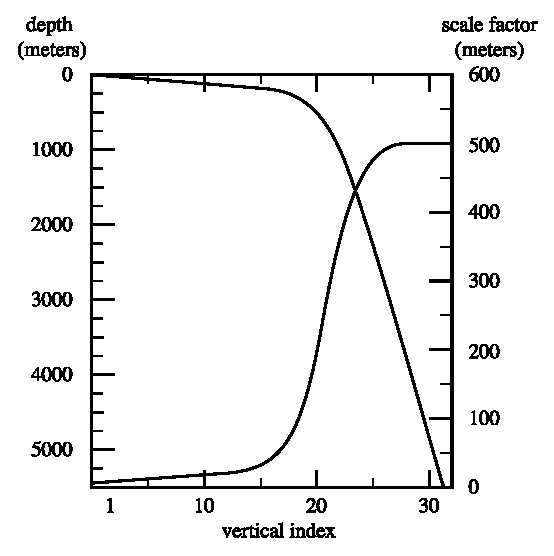
\includegraphics[width=0.90\textwidth]{Fig_zgr}
\caption{ \protect\label{fig:zgr}
  Default vertical mesh for ORCA2: 30 ocean levels (L30).
  Vertical level functions for (a) T-point depth and (b) the associated scale factor as computed from
  \autoref{eq:DOM_zgr_ana_1} using \autoref{eq:DOM_zgr_coef} in $z$-coordinate.}
\end{center}   \end{figure}
%>>>>>>>>>>>>>>>>>>>>>>>>>>>>

The reference coordinate transformation $z_0 (k)$ defines the arrays $gdept_0$ and $gdepw_0$ for
$t$- and $w$-points, respectively.
As indicated on \autoref{fig:index_vert} \jp{jpk} is the number of $w$-levels. $gdepw_0(1)$ is the ocean surface.
There are at most \jp{jpk}-1 $t$-points inside the ocean,
the additional $t$-point at $jk=jpk$ is below the sea floor and is not used.
The vertical location of $w$- and $t$-levels is defined from the analytic expression of the depth $z_0(k)$ whose
analytical derivative with respect to $k$ provides the vertical scale factors.
The user must provide the analytical expression of both $z_0$ and its first derivative with respect to $k$.
This is done in routine \mdl{domzgr} through statement functions,
using parameters provided in the \ngn{namcfg} namelist.

It is possible to define a simple regular vertical grid by giving zero stretching (\np{ppacr=0}).
In that case,
the parameters \jp{jpk} (number of $w$-levels) and \np{pphmax} (total ocean depth in meters) fully define the grid. 

For climate-related studies it is often desirable to concentrate the vertical resolution near the ocean surface.
The following function is proposed as a standard for a $z$-coordinate (with either full or partial steps): 
\begin{equation} \label{eq:DOM_zgr_ana_1}
\begin{split}
 z_0 (k) 	&= h_{sur} -h_0 \;k-\;h_1 \;\log \left[ {\,\cosh \left( {{(k-h_{th} )} / {h_{cr} }} \right)\,} \right] \\ 
 e_3^0 (k) 	&= \left| -h_0 -h_1 \;\tanh \left( {{(k-h_{th} )} / {h_{cr} }} \right) \right| 
\end{split}
\end{equation}
where $k=1$ to \jp{jpk} for $w$-levels and $k=1$ to $k=1$ for $T-$levels.
Such an expression allows us to define a nearly uniform vertical location of levels at the ocean top and bottom with
a smooth hyperbolic tangent transition in between (\autoref{fig:zgr}).

If the ice shelf cavities are opened (\np{ln\_isfcav}\forcode{ = .true.}), the definition of $z_0$ is the same.
However, definition of $e_3^0$ at $t$- and $w$-points is respectively changed to:
\begin{equation} \label{eq:DOM_zgr_ana_2}
\begin{split}
 e_3^T(k) &= z_W (k+1) - z_W (k)   \\
 e_3^W(k) &= z_T (k)   - z_T (k-1) \\
\end{split}
\end{equation}
This formulation decrease the self-generated circulation into the ice shelf cavity 
(which can, in extreme case, leads to blow up).\\

 
The most used vertical grid for ORCA2 has $10~m$ ($500~m)$ resolution in the surface (bottom) layers and
a depth which varies from 0 at the sea surface to a minimum of $-5000~m$.
This leads to the following conditions:
\begin{equation} \label{eq:DOM_zgr_coef}
\begin{split}
 e_3 (1+1/2)		&=10. \\ 
 e_3 (jpk-1/2)	&=500. \\ 
 z(1)			&=0. \\ 
 z(jpk)			&=-5000. \\ 
\end{split}
\end{equation}

With the choice of the stretching $h_{cr} =3$ and the number of levels \jp{jpk}=$31$,
the four coefficients $h_{sur}$, $h_{0}$, $h_{1}$, and $h_{th}$ in
\autoref{eq:DOM_zgr_ana_2} have been determined such that
\autoref{eq:DOM_zgr_coef} is satisfied, through an optimisation procedure using a bisection method.
For the first standard ORCA2 vertical grid this led to the following values:
$h_{sur} =4762.96$, $h_0 =255.58, h_1 =245.5813$, and $h_{th} =21.43336$.
The resulting depths and scale factors as a function of the model levels are shown in
\autoref{fig:zgr} and given in \autoref{tab:orca_zgr}.
Those values correspond to the parameters \np{ppsur}, \np{ppa0}, \np{ppa1}, \np{ppkth} in \ngn{namcfg} namelist. 

Rather than entering parameters $h_{sur}$, $h_{0}$, and $h_{1}$ directly, it is possible to recalculate them.
In that case the user sets \np{ppsur}\forcode{ = }\np{ppa0}\forcode{ = }\np{ppa1}\forcode{ = 999999}.,
in \ngn{namcfg} namelist, and specifies instead the four following parameters:
\begin{itemize}
\item
  \np{ppacr}=$h_{cr} $: stretching factor (nondimensional).
  The larger \np{ppacr}, the smaller the stretching.
  Values from $3$ to $10$ are usual.
\item
  \np{ppkth}=$h_{th} $: is approximately the model level at which maximum stretching occurs
  (nondimensional, usually of order 1/2 or 2/3 of \jp{jpk})
\item
  \np{ppdzmin}: minimum thickness for the top layer (in meters).
\item
  \np{pphmax}: total depth of the ocean (meters).
\end{itemize}
As an example, for the $45$ layers used in the DRAKKAR configuration those parameters are:
\jp{jpk}\forcode{ = 46}, \np{ppacr}\forcode{ = 9}, \np{ppkth}\forcode{ = 23.563},
\np{ppdzmin}\forcode{ = 6}m, \np{pphmax}\forcode{ = 5750}m.

%>>>>>>>>>>>>>>>>>>>>>>>>>>>>
\begin{table}     \begin{center} \begin{tabular}{c||r|r|r|r}
\hline
\textbf{LEVEL}& \textbf{gdept\_1d}& \textbf{gdepw\_1d}& \textbf{e3t\_1d }& \textbf{e3w\_1d  } \\ \hline
1	&	\textbf{  5.00}	&       0.00 &	\textbf{ 10.00} &	 10.00 \\	\hline
2	&	\textbf{15.00}	& 	  10.00 &	\textbf{ 10.00} &	 10.00 \\	\hline
3	&	\textbf{25.00}	&	  20.00 &	\textbf{ 10.00} & 	 10.00 \\	\hline
4	&	\textbf{35.01}	&	  30.00 & 	\textbf{ 10.01} & 	 10.00 \\	\hline
5	&	\textbf{45.01}	&	  40.01 &	\textbf{ 10.01} &	 10.01 \\	\hline
6	&	\textbf{55.03}	&	  50.02 &	\textbf{ 10.02} & 	 10.02 \\	\hline
7	&	\textbf{65.06}	&	  60.04 &	\textbf{ 10.04} &	 10.03 \\	\hline
8	&	\textbf{75.13}	&	  70.09 &	\textbf{ 10.09} &	 10.06 \\	\hline
9	&	\textbf{85.25}	&	  80.18 &	\textbf{ 10.17} &	 10.12 \\	\hline
10	& 	\textbf{95.49}	& 	  90.35 &	\textbf{ 10.33} &	 10.24 \\	\hline
11	& 	\textbf{105.97}	& 	 100.69 &	\textbf{ 10.65} &	 10.47 \\	\hline
12	& 	\textbf{116.90}	& 	 111.36 &	\textbf{ 11.27} &	 10.91 \\	\hline
13	& 	\textbf{128.70}	& 	 122.65 &	\textbf{ 12.47} &	 11.77 \\	\hline
14	& 	\textbf{142.20}	& 	 135.16 &	\textbf{ 14.78} &	 13.43 \\	\hline
15	& 	\textbf{158.96}	& 	 150.03 &	\textbf{ 19.23} &	 16.65 \\	\hline
16	& 	\textbf{181.96}	& 	 169.42 &	\textbf{ 27.66} &	 22.78 \\	\hline
17	& 	\textbf{216.65}	& 	 197.37 & 	\textbf{ 43.26} &	 34.30 \\ \hline
18	& 	\textbf{272.48}	& 	 241.13 & 	\textbf{ 70.88} &	 55.21 \\ \hline
19	& 	\textbf{364.30}	& 	 312.74 & 	\textbf{116.11} &	 90.99 \\ \hline
20	& 	\textbf{511.53}	& 	 429.72 & 	\textbf{181.55} & 	146.43 \\ \hline
21	& 	\textbf{732.20}	& 	 611.89 & 	\textbf{261.03} & 	220.35 \\ \hline
22	& 	\textbf{1033.22}&	 872.87 & 	\textbf{339.39} & 	301.42 \\ \hline
23	& 	\textbf{1405.70}&	1211.59 & \textbf{402.26} & 	373.31 \\ \hline
24	& 	\textbf{1830.89}&	1612.98 & \textbf{444.87} & 	426.00 \\ \hline
25	& 	\textbf{2289.77}&	2057.13 & \textbf{470.55} & 	459.47 \\ \hline
26	& 	\textbf{2768.24}&	2527.22 & \textbf{484.95} & 	478.83 \\ \hline
27	& 	\textbf{3257.48}&	3011.90 & \textbf{492.70} & 	489.44 \\ \hline
28	& 	\textbf{3752.44}&	3504.46 & \textbf{496.78} & 	495.07 \\ \hline
29	& 	\textbf{4250.40}&	4001.16 & \textbf{498.90} & 	498.02 \\ \hline
30	& 	\textbf{4749.91}&	4500.02 & \textbf{500.00} &	499.54 \\ \hline
31	& 	\textbf{5250.23}&	5000.00 &	\textbf{500.56} &	500.33 \\ \hline
\end{tabular} \end{center} 
\caption{ \protect\label{tab:orca_zgr}
  Default vertical mesh in $z$-coordinate for 30 layers ORCA2 configuration as computed from
  \autoref{eq:DOM_zgr_ana_2} using the coefficients given in \autoref{eq:DOM_zgr_coef}}
\end{table}
%>>>>>>>>>>>>>>>>>>>>>>>>>>>>

% -------------------------------------------------------------------------------------------------------------
%        z-coordinate with partial step
% -------------------------------------------------------------------------------------------------------------
\subsection{$Z$-coordinate with partial step (\protect\np{ln\_zps}\forcode{ = .true.})}
\label{subsec:DOM_zps}
%--------------------------------------------namdom-------------------------------------------------------

\nlst{namdom} 
%--------------------------------------------------------------------------------------------------------------

In $z$-coordinate partial step,
the depths of the model levels are defined by the reference analytical function $z_0 (k)$ as described in
the previous section, \emph{except} in the bottom layer.
The thickness of the bottom layer is allowed to vary as a function of geographical location $(\lambda,\varphi)$ to
allow a better representation of the bathymetry, especially in the case of small slopes
(where the bathymetry varies by less than one level thickness from one grid point to the next).
The reference layer thicknesses $e_{3t}^0$ have been defined in the absence of bathymetry.
With partial steps, layers from 1 to \jp{jpk}-2 can have a thickness smaller than $e_{3t}(jk)$.
The model deepest layer (\jp{jpk}-1) is allowed to have either a smaller or larger thickness than $e_{3t}(jpk)$:
the maximum thickness allowed is $2*e_{3t}(jpk-1)$.
This has to be kept in mind when specifying values in \ngn{namdom} namelist,
as the maximum depth \np{pphmax} in partial steps:
for example, with \np{pphmax}$=5750~m$ for the DRAKKAR 45 layer grid,
the maximum ocean depth allowed is actually $6000~m$ (the default thickness $e_{3t}(jpk-1)$ being $250~m$).
Two variables in the namdom namelist are used to define the partial step vertical grid.
The mimimum water thickness (in meters) allowed for a cell partially filled with bathymetry at level jk is
the minimum of \np{rn\_e3zps\_min} (thickness in meters, usually $20~m$) or $e_{3t}(jk)*$\np{rn\_e3zps\_rat}
(a fraction, usually 10\%, of the default thickness $e_{3t}(jk)$).

\gmcomment{ \colorbox{yellow}{Add a figure here of pstep especially at last ocean level }  }

% -------------------------------------------------------------------------------------------------------------
%        s-coordinate
% -------------------------------------------------------------------------------------------------------------
\subsection{$S$-coordinate (\protect\np{ln\_sco}\forcode{ = .true.})}
\label{subsec:DOM_sco}
%------------------------------------------nam_zgr_sco---------------------------------------------------
%
%\nlst{namzgr_sco} 
%--------------------------------------------------------------------------------------------------------------
Options are defined in \ngn{namzgr\_sco}.
In $s$-coordinate (\np{ln\_sco}\forcode{ = .true.}), the depth and thickness of the model levels are defined from
the product of a depth field and either a stretching function or its derivative, respectively:

\begin{equation} \label{eq:DOM_sco_ana}
\begin{split}
 z(k) 		&= h(i,j) \; z_0(k)	\\
 e_3(k)	&= h(i,j) \; z_0'(k)
\end{split}
\end{equation}

where $h$ is the depth of the last $w$-level ($z_0(k)$) defined at the $t$-point location in the horizontal and
$z_0(k)$ is a function which varies from $0$ at the sea surface to $1$ at the ocean bottom.
The depth field $h$ is not necessary the ocean depth,
since a mixed step-like and bottom-following representation of the topography can be used
(\autoref{fig:z_zps_s_sps}d-e) or an envelop bathymetry can be defined (\autoref{fig:z_zps_s_sps}f).
The namelist parameter \np{rn\_rmax} determines the slope at which
the terrain-following coordinate intersects the sea bed and becomes a pseudo z-coordinate. 
The coordinate can also be hybridised by specifying \np{rn\_sbot\_min} and \np{rn\_sbot\_max} as
the minimum and maximum depths at which the terrain-following vertical coordinate is calculated.

Options for stretching the coordinate are provided as examples,
but care must be taken to ensure that the vertical stretch used is appropriate for the application.

The original default NEMO s-coordinate stretching is available if neither of the other options are specified as true
(\np{ln\_s\_SH94}\forcode{ = .false.} and \np{ln\_s\_SF12}\forcode{ = .false.}). 
This uses a depth independent $\tanh$ function for the stretching \citep{Madec_al_JPO96}:

\begin{equation}
  z = s_{min}+C\left(s\right)\left(H-s_{min}\right)
  \label{eq:SH94_1}
\end{equation}

where $s_{min}$ is the depth at which the $s$-coordinate stretching starts and
allows a $z$-coordinate to placed on top of the stretched coordinate,
and $z$ is the depth (negative down from the asea surface).

\begin{equation}
  s = -\frac{k}{n-1} \quad \text{ and } \quad 0 \leq k \leq n-1
  \label{eq:DOM_s}
\end{equation}

\begin{equation} \label{eq:DOM_sco_function}
\begin{split}
C(s)	&=  \frac{ \left[	  \tanh{ \left( \theta \, (s+b) \right)} 
	  	 			- \tanh{ \left(  \theta \, b      \right)}  \right]}
		      {2\;\sinh \left( \theta \right)}
\end{split}
\end{equation}

A stretching function,
modified from the commonly used \citet{Song_Haidvogel_JCP94} stretching (\np{ln\_s\_SH94}\forcode{ = .true.}),
is also available and is more commonly used for shelf seas modelling:

\begin{equation}
  C\left(s\right) =   \left(1 - b \right)\frac{ \sinh\left( \theta s\right)}{\sinh\left(\theta\right)} +      \\
  b\frac{ \tanh \left[ \theta \left(s + \frac{1}{2} \right)\right] - \tanh\left(\frac{\theta}{2}\right)}{ 2\tanh\left (\frac{\theta}{2}\right)}
  \label{eq:SH94_2}
\end{equation}

%>>>>>>>>>>>>>>>>>>>>>>>>>>>>
\begin{figure}[!ht]    \begin{center}
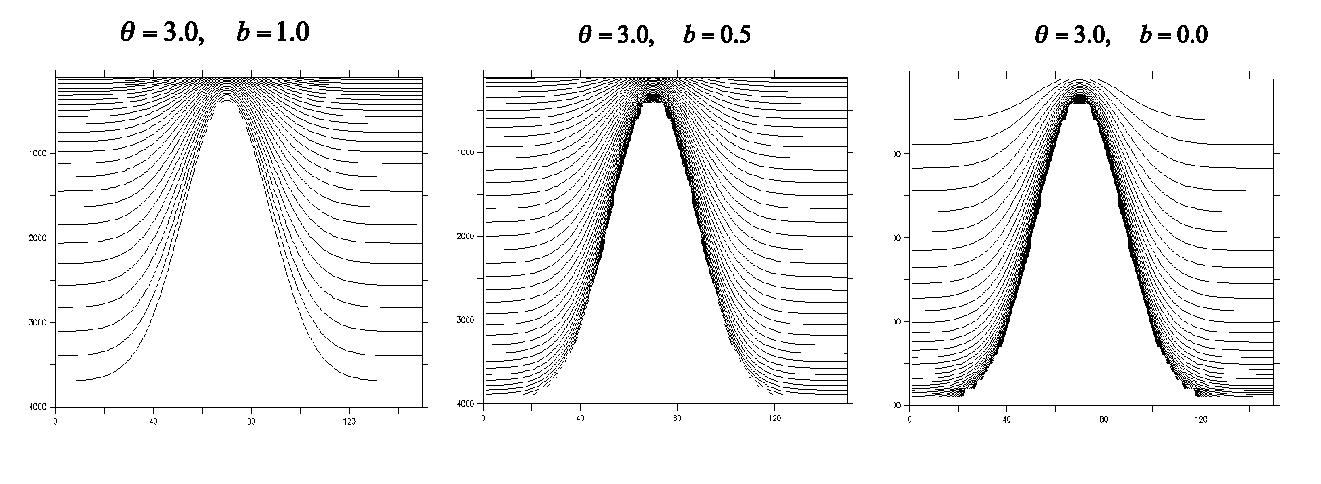
\includegraphics[width=1.0\textwidth]{Fig_sco_function}
\caption{  \protect\label{fig:sco_function}
  Examples of the stretching function applied to a seamount;
  from left to right: surface, surface and bottom, and bottom intensified resolutions}
\end{center}   \end{figure}
%>>>>>>>>>>>>>>>>>>>>>>>>>>>>

where $H_c$ is the critical depth (\np{rn\_hc}) at which
the coordinate transitions from pure $\sigma$ to the stretched coordinate,
and $\theta$ (\np{rn\_theta}) and $b$ (\np{rn\_bb}) are the surface and bottom control parameters such that
$0\leqslant \theta \leqslant 20$, and $0\leqslant b\leqslant 1$.
$b$ has been designed to allow surface and/or bottom increase of the vertical resolution
(\autoref{fig:sco_function}).

Another example has been provided at version 3.5 (\np{ln\_s\_SF12}) that allows a fixed surface resolution in
an analytical terrain-following stretching \citet{Siddorn_Furner_OM12}.
In this case the a stretching function $\gamma$ is defined such that:

\begin{equation}
z = -\gamma h \quad \text{ with } \quad 0 \leq \gamma \leq 1
\label{eq:z}
\end{equation}

The function is defined with respect to $\sigma$, the unstretched terrain-following coordinate:

\begin{equation} \label{eq:DOM_gamma_deriv}
\gamma= A\left(\sigma-\frac{1}{2}\left(\sigma^{2}+f\left(\sigma\right)\right)\right)+B\left(\sigma^{3}-f\left(\sigma\right)\right)+f\left(\sigma\right)
\end{equation}

Where:
\begin{equation} \label{eq:DOM_gamma}
f\left(\sigma\right)=\left(\alpha+2\right)\sigma^{\alpha+1}-\left(\alpha+1\right)\sigma^{\alpha+2} \quad \text{ and } \quad \sigma = \frac{k}{n-1} 
\end{equation}

This gives an analytical stretching of $\sigma$ that is solvable in $A$ and $B$ as a function of
the user prescribed stretching parameter $\alpha$ (\np{rn\_alpha}) that stretches towards
the surface ($\alpha > 1.0$) or the bottom ($\alpha < 1.0$) and
user prescribed surface (\np{rn\_zs}) and bottom depths.
The bottom cell depth in this example is given as a function of water depth:

\begin{equation} \label{eq:DOM_zb}
Z_b= h a + b
\end{equation}

where the namelist parameters \np{rn\_zb\_a} and \np{rn\_zb\_b} are $a$ and $b$ respectively.

%>>>>>>>>>>>>>>>>>>>>>>>>>>>>
\begin{figure}[!ht]
   \includegraphics[width=1.0\textwidth]{Fig_DOM_compare_coordinates_surface}
   \caption{
     A comparison of the \citet{Song_Haidvogel_JCP94} $S$-coordinate (solid lines),
     a 50 level $Z$-coordinate (contoured surfaces) and
     the \citet{Siddorn_Furner_OM12} $S$-coordinate (dashed lines) in
     the surface 100m for a idealised bathymetry that goes from 50m to 5500m depth.
     For clarity every third coordinate surface is shown.}
    \label{fig:fig_compare_coordinates_surface}
\end{figure}
%>>>>>>>>>>>>>>>>>>>>>>>>>>>>

This gives a smooth analytical stretching in computational space that is constrained to
given specified surface and bottom grid cell thicknesses in real space.
This is not to be confused with the hybrid schemes that
superimpose geopotential coordinates on terrain following coordinates thus
creating a non-analytical vertical coordinate that
therefore may suffer from large gradients in the vertical resolutions.
This stretching is less straightforward to implement than the \citet{Song_Haidvogel_JCP94} stretching,
but has the advantage of resolving diurnal processes in deep water and has generally flatter slopes.

As with the \citet{Song_Haidvogel_JCP94} stretching the stretch is only applied at depths greater than
the critical depth $h_c$.
In this example two options are available in depths shallower than $h_c$,
with pure sigma being applied if the \np{ln\_sigcrit} is true and pure z-coordinates if it is false
(the z-coordinate being equal to the depths of the stretched coordinate at $h_c$).

Minimising the horizontal slope of the vertical coordinate is important in terrain-following systems as
large slopes lead to hydrostatic consistency.
A hydrostatic consistency parameter diagnostic following \citet{Haney1991} has been implemented,
and is output as part of the model mesh file at the start of the run.

% -------------------------------------------------------------------------------------------------------------
%        z*- or s*-coordinate
% -------------------------------------------------------------------------------------------------------------
\subsection{$Z^*$- or $S^*$-coordinate (\protect\np{ln\_linssh}\forcode{ = .false.}) }
\label{subsec:DOM_zgr_star}

This option is described in the Report by Levier \textit{et al.} (2007), available on the \NEMO web site. 

%gm% key advantage: minimise the diffusion/dispertion associated with advection in response to high frequency surface disturbances

% -------------------------------------------------------------------------------------------------------------
%        level bathymetry and mask 
% -------------------------------------------------------------------------------------------------------------
\subsection{Level bathymetry and mask}
\label{subsec:DOM_msk}

Whatever the vertical coordinate used,
the model offers the possibility of representing the bottom topography with steps that
follow the face of the model cells (step like topography) \citep{Madec_al_JPO96}.
The distribution of the steps in the horizontal is defined in a 2D integer array, mbathy,
which gives the number of ocean levels ($i.e.$ those that are not masked) at each $t$-point.
mbathy is computed from the meter bathymetry using the definiton of gdept as
the number of $t$-points which gdept $\leq$ bathy.

Modifications of the model bathymetry are performed in the \textit{bat\_ctl} routine (see \mdl{domzgr} module) after
mbathy is computed.
Isolated grid points that do not communicate with another ocean point at the same level are eliminated.

As for the representation of bathymetry, a 2D integer array, misfdep, is created.
misfdep defines the level of the first wet $t$-point.
All the cells between $k=1$ and $misfdep(i,j)-1$ are masked.
By default, misfdep(:,:)=1 and no cells are masked.

In case of ice shelf cavities, modifications of the model bathymetry and ice shelf draft into 
the cavities are performed in the \textit{zgr\_isf} routine.
The compatibility between ice shelf draft and bathymetry is checked. 
All the locations where the isf cavity is thinnest than \np{rn\_isfhmin} meters are grounded ($i.e.$ masked). 
If only one cell on the water column is opened at $t$-, $u$- or $v$-points,
the bathymetry or the ice shelf draft is dug to fit this constrain.
If the incompatibility is too strong (need to dig more than 1 cell), the cell is masked.\\ 

From the \textit{mbathy} and \textit{misfdep} array, the mask fields are defined as follows:
\begin{align*}
tmask(i,j,k) &= \begin{cases}   \; 0&   \text{ if $k < misfdep(i,j) $ } \\
                                \; 1&   \text{ if $misfdep(i,j) \leq k\leq mbathy(i,j)$  }    \\
                                \; 0&   \text{ if $k > mbathy(i,j)$  }    \end{cases}     \\
umask(i,j,k) &=         \; tmask(i,j,k) \ * \ tmask(i+1,j,k)	\\
vmask(i,j,k) &=         \; tmask(i,j,k) \ * \ tmask(i,j+1,k)	\\
fmask(i,j,k) &=         \; tmask(i,j,k) \ * \ tmask(i+1,j,k)	\\
             &    \ \ \, * tmask(i,j,k) \ * \ tmask(i+1,j,k) \\
wmask(i,j,k) &=         \; tmask(i,j,k) \ * \ tmask(i,j,k-1) \text{ with } wmask(i,j,1) = tmask(i,j,1) 
\end{align*}

Note that, without ice shelves cavities,
masks at $t-$ and $w-$points are identical with the numerical indexing used (\autoref{subsec:DOM_Num_Index}).
Nevertheless, $wmask$ are required with ocean cavities to deal with the top boundary (ice shelf/ocean interface) 
exactly in the same way as for the bottom boundary. 

The specification of closed lateral boundaries requires that at least
the first and last rows and columns of the \textit{mbathy} array are set to zero.
In the particular case of an east-west cyclical boundary condition,
\textit{mbathy} has its last column equal to the second one and its first column equal to the last but one 
(and so too the mask arrays) (see \autoref{fig:LBC_jperio}).


% ================================================================
% Domain: Initial State (dtatsd & istate)
% ================================================================
\section{Initial state (\protect\mdl{istate} and \protect\mdl{dtatsd})}
\label{sec:DTA_tsd}
%-----------------------------------------namtsd-------------------------------------------

\nlst{namtsd} 
%------------------------------------------------------------------------------------------

Options are defined in \ngn{namtsd}.
By default, the ocean start from rest (the velocity field is set to zero) and the initialization of temperature and salinity fields is controlled through the \np{ln\_tsd\_ini} namelist parameter.
\begin{description}
\item[\np{ln\_tsd\_init}\forcode{ = .true.}]
  use a T and S input files that can be given on the model grid itself or on their native input data grid.
  In the latter case,
  the data will be interpolated on-the-fly both in the horizontal and the vertical to the model grid
  (see \autoref{subsec:SBC_iof}).
  The information relative to the input files are given in the \np{sn\_tem} and \np{sn\_sal} structures.
  The computation is done in the \mdl{dtatsd} module.
\item[\np{ln\_tsd\_init}\forcode{ = .false.}]
  use constant salinity value of 35.5 psu and an analytical profile of temperature (typical of the tropical ocean),
  see \rou{istate\_t\_s} subroutine called from \mdl{istate} module.
\end{description}
\end{document}
